\section{Discussion}
\label{sec:discussion}

\paragraph{When does simplification appear low-risk in this case study?}
Our results across three evaluation dimensions indicate that
MDL-to-UsdPreviewSurface conversion can be low-risk for tested assets whose
appearance is dominated by standard PBR channels (diffuse albedo, roughness,
metallic, normal). For such assets, we observe PSNR $>$ 35\,dB, SSIM $>$ 0.99, CLIP
similarity $>$ 0.92. Caution is
warranted for materials that rely on multi-layer MDL effects --- procedural
noise textures, specular coatings, and anisotropic reflectance --- where
per-viewpoint PSNR can drop below 25\,dB and DINOv2 similarity below 0.60. We
recommend that practitioners validate such materials individually using the
feature-level metrics introduced here, which are more sensitive to perceptually
relevant differences than pixel-level metrics alone. The material-effect
baseline in Table~\ref{tab:material_effect_risk_matrix} sharpens this guideline:
covered GRScenes bins support bounded selected qualitative evidence, but
clearcoat and procedural texture remain explicitly risk-gated rather than
converted into broad success claims.

\paragraph{The within-simulation rendering gap.}
Much prior work has focused on the sim-to-real
gap~\cite{Tobin2017Domain,Tremblay2018Training,Zhao2020Sim,Garcia2023Robust}:
the distribution shift between synthetic and real images. Our work highlights a
complementary and less-studied phenomenon --- the \emph{within-simulation
rendering gap} --- arising from differences in material representation within
the same renderer. When converting MDL to UsdPreviewSurface, geometry, lighting,
and camera parameters remain identical; only the material shader changes. The
resulting image differences are therefore a controlled measure of how much visual
information is lost when reducing a high-fidelity material model to a simpler
one. Our finding that this gap is small (SSIM $>$ 0.99, CLIP $>$ 0.92) for the
tested standard-PBR furniture assets leads us to hypothesize that, for many practical
applications, the within-simulation gap introduced by material simplification
is small relative to typical sim-to-real gaps reported in the literature.

\paragraph{Interoperability versus fidelity.}
The performance story is workload-dependent. In our shallow single-object RTX
path-tracing benchmark, FPS and GPU memory are nearly identical between MDL and
UsdPreviewSurface, and the only visible difference is reduced first-load
latency variability. In contrast, the supplemental GRScenes whole-scene startup
runs to a substantial gain for noMDL: time to a fully warmed ready-to-render
state drops from 52.0\,s to 13.7\,s, and post-load GPU memory decreases by
roughly 200\,MB. The fact that this gap emerges primarily during the post-open warm-up phase
rather than the raw \texttt{open\_stage} call suggests that material
initialization and early-frame settling dominate startup cost once scene scale
and shader complexity become substantial. The clearest general benefit in this
study remains interoperability: UsdPreviewSurface materials are supported by
standard USD viewers, web-based 3D platforms, and the glTF/GLB export path,
none of which can interpret NVIDIA's proprietary MDL shaders. Our results
quantify the visual cost of this interoperability gain: a mean LPIPS increase
of 0.020 and a DINOv2 cosine similarity of 0.872. For synthetic data pipelines
where downstream models operate on features rather than pixels, this trade-off
may be favorable, but it should still be gated by task-specific checks.

\paragraph{VLM grounding requires a stricter gate.}
The GRScenes results show why feature similarity and qualitative scene fidelity
are not enough for language-conditioned grounding claims. In the clean PASS
pool, Gemma4 preserves answer accuracy across material conditions, but its
point hits remain imperfect and slightly lower after conversion. Qwen2.5-VL is
more sensitive to response format and coordinate interpretation: raw-image
points score better than normalized-1000 scoring even though the prompt asks
for normalized coordinates. In the expanded 30-pair stress set, Gemma4 remains
stable under the frozen normalized-1000 protocol, while Qwen shows answer and
raw-point degradation on converted renders and still does not follow the same
coordinate semantics. Because the stress cameras are target-centered and the
set is category-imbalanced, these point-hit results should not be read as
general localization accuracy. Their main value is to expose protocol
sensitivity under a controlled material-shift intervention. This does not imply
that conversion generally harms VLM grounding; rather, it shows that the effect
is model- and protocol-dependent, and that clean-preservation pools must be
separated from material-shift stress tests.

\paragraph{Why DINOv2 is more sensitive than CLIP.}
Figure~\ref{fig:tsne_dino} provides a t-SNE visualization of DINOv2 embeddings
for all 48 rendered images. MDL and UsdPreviewSurface renderings of the same
scene cluster tightly together, confirming that material simplification produces
a smaller feature-space perturbation than the inter-scene variation.

\begin{figure}[t]
\centering
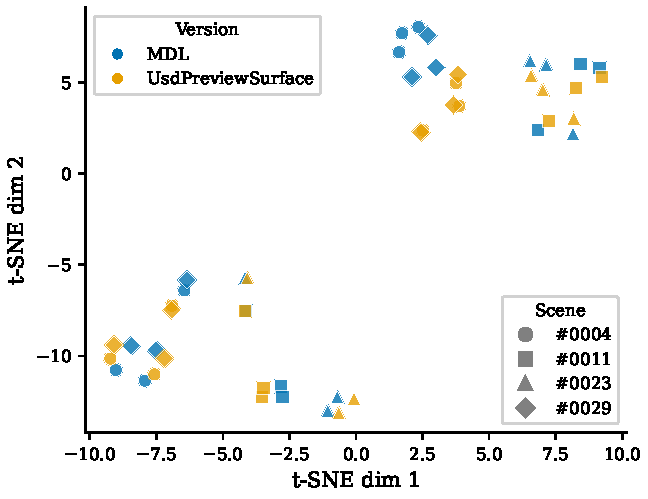
\includegraphics[width=\linewidth]{figures/fig_tsne_dino.pdf}
\caption{t-SNE projection of DINOv2 ViT-B/14 embeddings for all 48 images
(24 MDL + 24 UsdPreviewSurface), computed with perplexity\,=\,12,
learning rate\,=\,auto, and PCA initialization (random seed\,=\,42).
Same-scene pairs cluster tightly, indicating that the within-material
perturbation is small relative to inter-scene variation in the DINOv2
feature space.}
\label{fig:tsne_dino}
\end{figure}

CLIP's contrastive language--image pre-training~\cite{Radford2021Learning}
optimizes for high-level semantic alignment between images and text, producing
representations that are naturally invariant to low-level appearance changes
such as texture detail, specular highlights, and subtle color shifts. DINOv2's
self-supervised objective~\cite{Oquab2023DINOv2}, by contrast, preserves
fine-grained spatial and textural features, making it more sensitive to exactly
the kind of local appearance differences that material simplification
introduces. The gap between CLIP (0.925) and DINOv2 (0.872) similarity thus
reflects the granularity of each model's learned representations rather than a
deficiency in the conversion. Practitioners should select the appropriate
metric based on their downstream task: CLIP similarity is most relevant for
tasks relying on high-level semantics (e.g., image--text retrieval,
classification), while DINOv2 similarity better captures texture-level fidelity
relevant to dense prediction tasks (e.g., segmentation, depth estimation).

\paragraph{Practical recommendations.}
Based on our findings, we offer the following guidelines for synthetic data
practitioners working with Isaac Sim assets:

\begin{table*}[t]
\centering
\caption{Lightweight safe-conversion recommender derived from the material-effect risk matrix. The rules are reviewer guidance from the selected evidence rather than a learned classifier.}
\label{tab:material_safe_conversion_recommender}
\scriptsize
\resizebox{\textwidth}{!}{%
\begin{tabular}{llll}
\toprule
\textbf{Effect} & \textbf{Risk} & \textbf{ConvertAsset action} & \textbf{Paper use} \\
\midrule
clearcoat & manual\_review\_high & manual\_visual\_review\_of\_preview\_approximation & selected\_failure\_case\_only \\
opacity\_transparency & selected\_low & convert\_with\_static\_check\_and\_selected\_visual\_review & selected\_evidence\_only \\
emission & selected\_low & convert\_with\_static\_check\_and\_selected\_visual\_review & selected\_evidence\_only \\
procedural\_texture & high & keep\_mdl\_or\_bake\_before\_reporting\_preservation & limitation\_or\_investigation\_only \\
normal\_bump & selected\_low & convert\_with\_static\_check\_and\_selected\_visual\_review & selected\_evidence\_only \\
displacement\_height & selected\_low & convert\_with\_static\_check\_and\_selected\_visual\_review & selected\_evidence\_only \\
\bottomrule
\end{tabular}%
}
\end{table*}


Table~\ref{tab:material_safe_conversion_recommender} converts the
material-effect risk matrix into a lightweight rule table. It is intentionally
not a learned classifier: each action is tied to the selected evidence above.
The table is useful as reviewer-facing decision support because it separates
bounded-low covered bins from clearcoat manual-review risk and procedural
texture preservation risk.

\begin{enumerate}
    \item \textbf{Use conversion as a candidate default only after task-specific
    checks} for assets with standard PBR materials. In our furniture case
    study, the quality loss is small and the interoperability benefits are
    significant, but this does not remove the need for downstream validation.
    \item \textbf{Validate complex materials} using CLIP and DINOv2 cosine
    similarity as quick diagnostic metrics before deploying converted assets in
    training pipelines.
    \item \textbf{Keep effect-specific claim boundaries.} In our current
    ConvertAsset-vs-NVIDIA matrix, opacity/transparency, emission, normal/bump,
    and displacement/height have bounded selected qualitative support; clearcoat
    is a selected NVIDIA target-loss failure case; procedural texture remains a
    limitation case for both converted conditions.
    \item \textbf{Use low CLIP similarity as a manual-review trigger.} In this
    dataset, the single pair below 0.85 corresponds to a viewpoint with complex
    specular effects, suggesting that unusually low CLIP similarity merits
    visual inspection rather than serving as a universal acceptance threshold.
    \item \textbf{Monitor low DINOv2 similarity for texture-sensitive tasks.}
    In our dataset, values below 0.80 occur only for viewpoints with complex
    specular effects. We therefore treat this range as a cautionary signal for
    manual validation, not as a hard deployment rule.
    \item \textbf{Add VLM-specific acceptance gates} before using converted
    renders as embodied-language benchmark evidence. Answer accuracy, point
    grounding, coordinate conventions, and visual-QA filtering should be
    reported separately.
\end{enumerate}
These recommendations are heuristic signals derived from furniture assets with
predominantly wood, metal, and fabric materials. Validation on diverse object
categories (e.g., transparent, organic, or highly specular surfaces) is needed
before broader generalization.
